\documentclass[border=8pt]{standalone}
\usepackage[T1]{fontenc}
\usepackage[utf8]{inputenc}
\usepackage{tikz}
\usetikzlibrary{arrows.meta}
\begin{document}
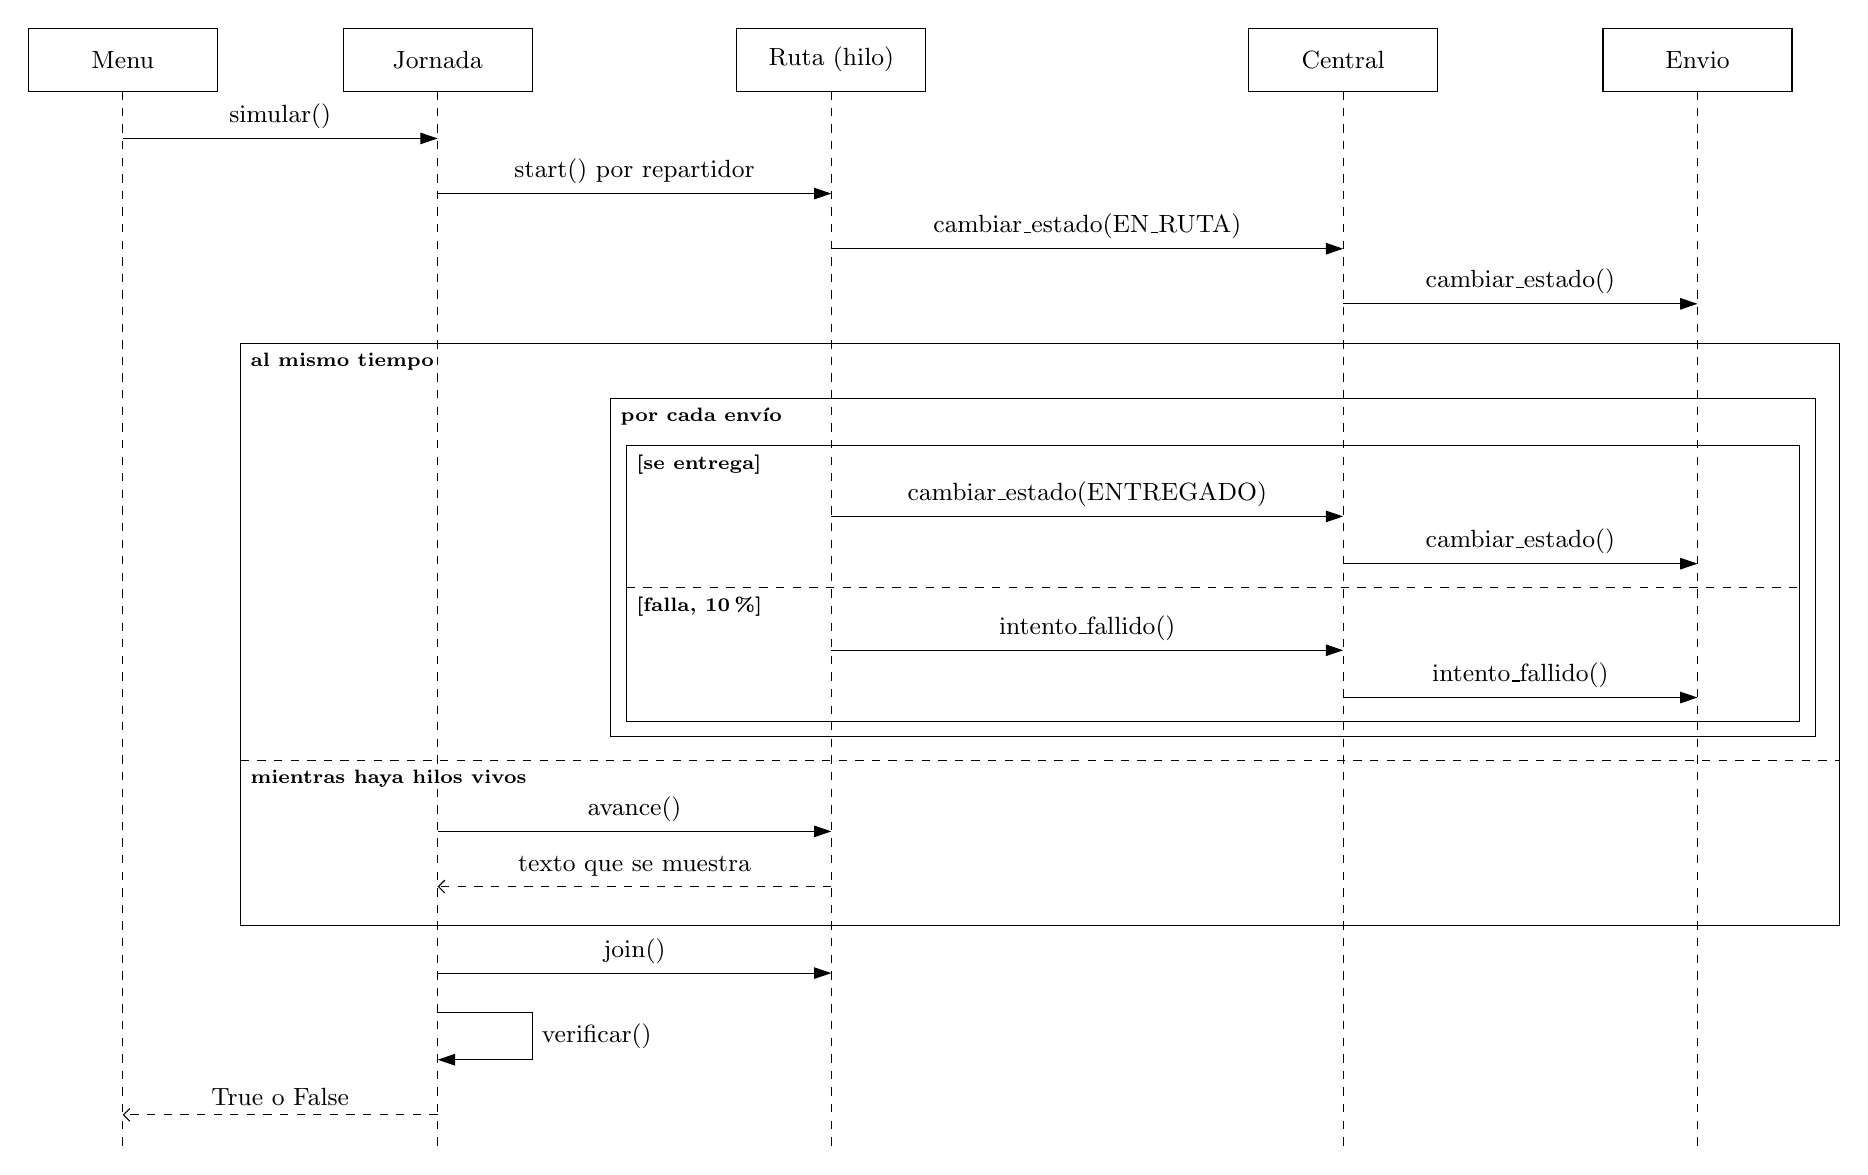
\begin{tikzpicture}[font=\small,o/.style={draw,minimum width=2.4cm,minimum height=8mm},
  ll/.style={dashed},m/.style={-{Triangle[length=2.2mm]}},r/.style={dashed,-{Straight Barb}},
  t/.style={anchor=north west,font=\scriptsize\bfseries}]
\foreach \x/\n in {0/Menu,4/Jornada,9/Ruta (hilo),15.5/Central,20/Envio}{
  \node[o] at (\x,0) {\n};
  \draw[ll] (\x,-0.4) -- (\x,-13.8);
}
\draw[m] (0,-1) -- node[above]{simular()} (4,-1);
\draw[m] (4,-1.7) -- node[above]{start() por repartidor} (9,-1.7);
\draw[m] (9,-2.4) -- node[above]{cambiar\_estado(EN\_RUTA)} (15.5,-2.4);
\draw[m] (15.5,-3.1) -- node[above]{cambiar\_estado()} (20,-3.1);
\draw (1.5,-3.6) rectangle (21.8,-11);
\node[t] at (1.5,-3.6) {al mismo tiempo};
\draw (6.2,-4.3) rectangle (21.5,-8.6);
\node[t] at (6.2,-4.3) {por cada envío};
\draw (6.4,-4.9) rectangle (21.3,-8.4);
\node[t] at (6.4,-4.9) {[se entrega]};
\draw[m] (9,-5.8) -- node[above]{cambiar\_estado(ENTREGADO)} (15.5,-5.8);
\draw[m] (15.5,-6.4) -- node[above]{cambiar\_estado()} (20,-6.4);
\draw[dashed] (6.4,-6.7) -- (21.3,-6.7);
\node[t] at (6.4,-6.7) {[falla, 10\,\%]};
\draw[m] (9,-7.5) -- node[above]{intento\_fallido()} (15.5,-7.5);
\draw[m] (15.5,-8.1) -- node[above]{intento\_fallido()} (20,-8.1);
\draw[dashed] (1.5,-8.9) -- (21.8,-8.9);
\node[t] at (1.5,-8.9) {mientras haya hilos vivos};
\draw[m] (4,-9.8) -- node[above]{avance()} (9,-9.8);
\draw[r] (9,-10.5) -- node[above]{texto que se muestra} (4,-10.5);
\draw[m] (4,-11.6) -- node[above]{join()} (9,-11.6);
\draw[m] (4,-12.1) -- (5.2,-12.1) -- (5.2,-12.7) -- (4,-12.7);
\node[anchor=west] at (5.2,-12.4) {verificar()};
\draw[r] (4,-13.4) -- node[above]{True o False} (0,-13.4);
\end{tikzpicture}
\end{document}
